%%%%%%%%%%%%%%%%%%%%%%%%%%%%%%%%%%%%%%%%%%%%%%%%%%%%%%%%%%%%
%% Chapter 2 — Fundamentals and Related Work (12–18 pages)
%% Purpose: provide only the theory and literature needed to
%% understand the research choices, then end with the
%% unresolved gap addressed by the thesis.
%%%%%%%%%%%%%%%%%%%%%%%%%%%%%%%%%%%%%%%%%%%%%%%%%%%%%%%%%%%%
\chapter{Fundamentals and Related Work}
\label{chap:fundamentals}

Chapter~\ref{chap:introduction} argued that precise task-space tracking
with a hydraulic mowing arm is limited less by kinematics than by the
actuator. The path from a valve command to actual cylinder motion is
nonlinear and load dependent, and it differs from one machine, season, or
attachment to the next. This chapter collects the background needed to
judge that argument and to understand the design decisions made later in
the thesis. Section~\ref{sec:fund:actuation} introduces the machine class
and its electro-hydraulic actuation. Section~\ref{sec:fund:kinematics}
recalls the kinematic tools behind the classical controller, and
Section~\ref{sec:fund:conventional-control} reviews how conventional
model-based control deals with hydraulic uncertainty. The following
sections turn to the learning methods this work builds on: data-driven
dynamics models and the pitfalls of identifying them from closed-loop data
(Section~\ref{sec:fund:learned-dynamics}), reduced-order and grey-box
modeling (Section~\ref{sec:fund:rom}), domain randomization and latent
adaptation (Section~\ref{sec:fund:domain-randomization}), and policy
optimization with structured priors
(Section~\ref{sec:fund:rl-residual}).
Section~\ref{sec:fund:gap} then states the gap that remains and how the
three control stacks of this thesis (\ppoROM, \ppoIDFD, and
\ppoIDAAMFD) address it. Only material that is
needed for the later chapters is included. The concrete system definition
and problem formulation follow in Chapter~\ref{chap:system}.

\section{Manipulator Actuation and Control Fundamentals}
\label{sec:fund:actuation}

\subsection{Application Context and Implement Carriers}

The machine studied in this thesis belongs to a class that is easy to
overlook because it is so common: hydraulic booms mounted on road-going
implement carriers, doing repetitive maintenance work along traffic
infrastructure. Figure~\ref{fig:fund:fme500} shows the concrete instance,
the MULAG FME~500 front mower on a Unimog
carrier~\cite{mulag2024fme500}. A multi-link boom carries a
$\unit[1.2]{m}$ flail mowing head to the roadside verge, reaches up to
about $\unit[6.5]{m}$ to either side of the vehicle, and must hold the
head in a shallow band above the ground while the vehicle creeps along
the road. The working envelope in Figure~\ref{fig:fund:fme500}(b) makes
the difficulty concrete. The same arm that mows a flat verge beside the
wheels must also reach over guardrails, down embankments to about
$\unit[3]{m}$ below road level, and up to $\unit[8]{m}$ for hedge work,
with the same linkage and the same operator. In practice, head height,
tilt, and lateral position are adjusted continuously by a human through
open-loop joystick commands. It is skilled and fatiguing work, done while
also driving the vehicle. Automating the tracking part of this task is
the practical motivation of this thesis.

\begin{figure}[tb]
  \centering
  \begin{subfigure}[b]{.58\linewidth}
    \centering
    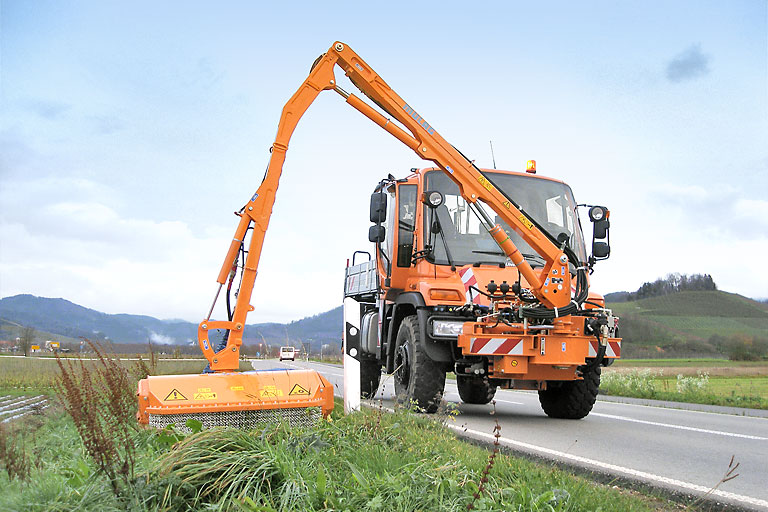
\includegraphics[width=\linewidth]{images/fme500_operation}
    \caption{}
    \label{fig:fund:fme500-photo}
  \end{subfigure}
  \hfill
  \begin{subfigure}[b]{.38\linewidth}
    \centering
    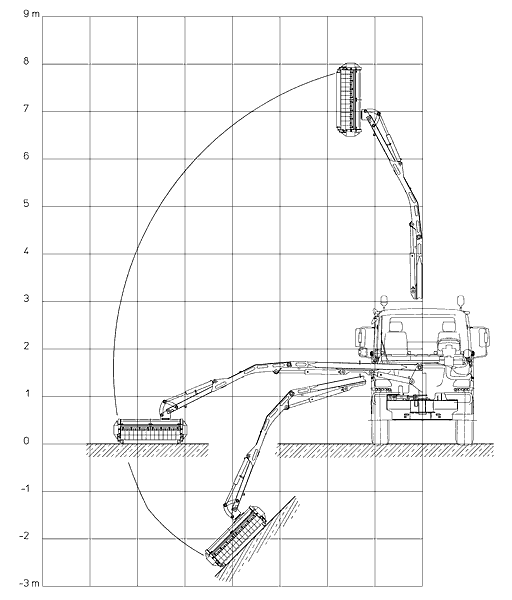
\includegraphics[width=.82\linewidth]{images/fme500_reach_diagram}
    \caption{}
    \label{fig:fund:fme500-reach}
  \end{subfigure}
  \caption{The plant considered in this thesis. (a)~MULAG FME~500 front
  mower on a Unimog implement carrier during roadside mowing. The
  multi-link hydraulic boom holds the flail head against the verge while
  the vehicle drives. (b)~Manufacturer's working envelope of the boom,
  spanning roughly $\unit[8]{m}$ of height and reaching below road level
  for embankment mowing. Images: MULAG Fahrzeugwerk~\cite{mulag2024fme500}.}
  \label{fig:fund:fme500}
\end{figure}

Hydraulic actuation dominates this machine class for reasons that remain
valid despite the rise of electric drives. Cylinders deliver very high
force from small, rugged, and inexpensive components; they tolerate shock
loads such as the mowing head striking a curbstone; and the carrier
vehicle already provides hydraulic power through its power take-off. The
price is paid in controllability. An electric joint drive responds to
current within milliseconds and nearly linearly. A hydraulic cylinder
responds through a chain of nonlinear energy conversions whose effective
gain can change by an order of magnitude across the workspace. Mattila et
al.~\cite{mattila2017survey} survey two decades of research on this
tension between the force density of hydraulic manipulators and the
difficulty of controlling them precisely.

\subsection{The Electro-Hydraulic Actuation Chain}
\label{sec:fund:actuation-chain}

\begin{figure}[tb]
  \centering
  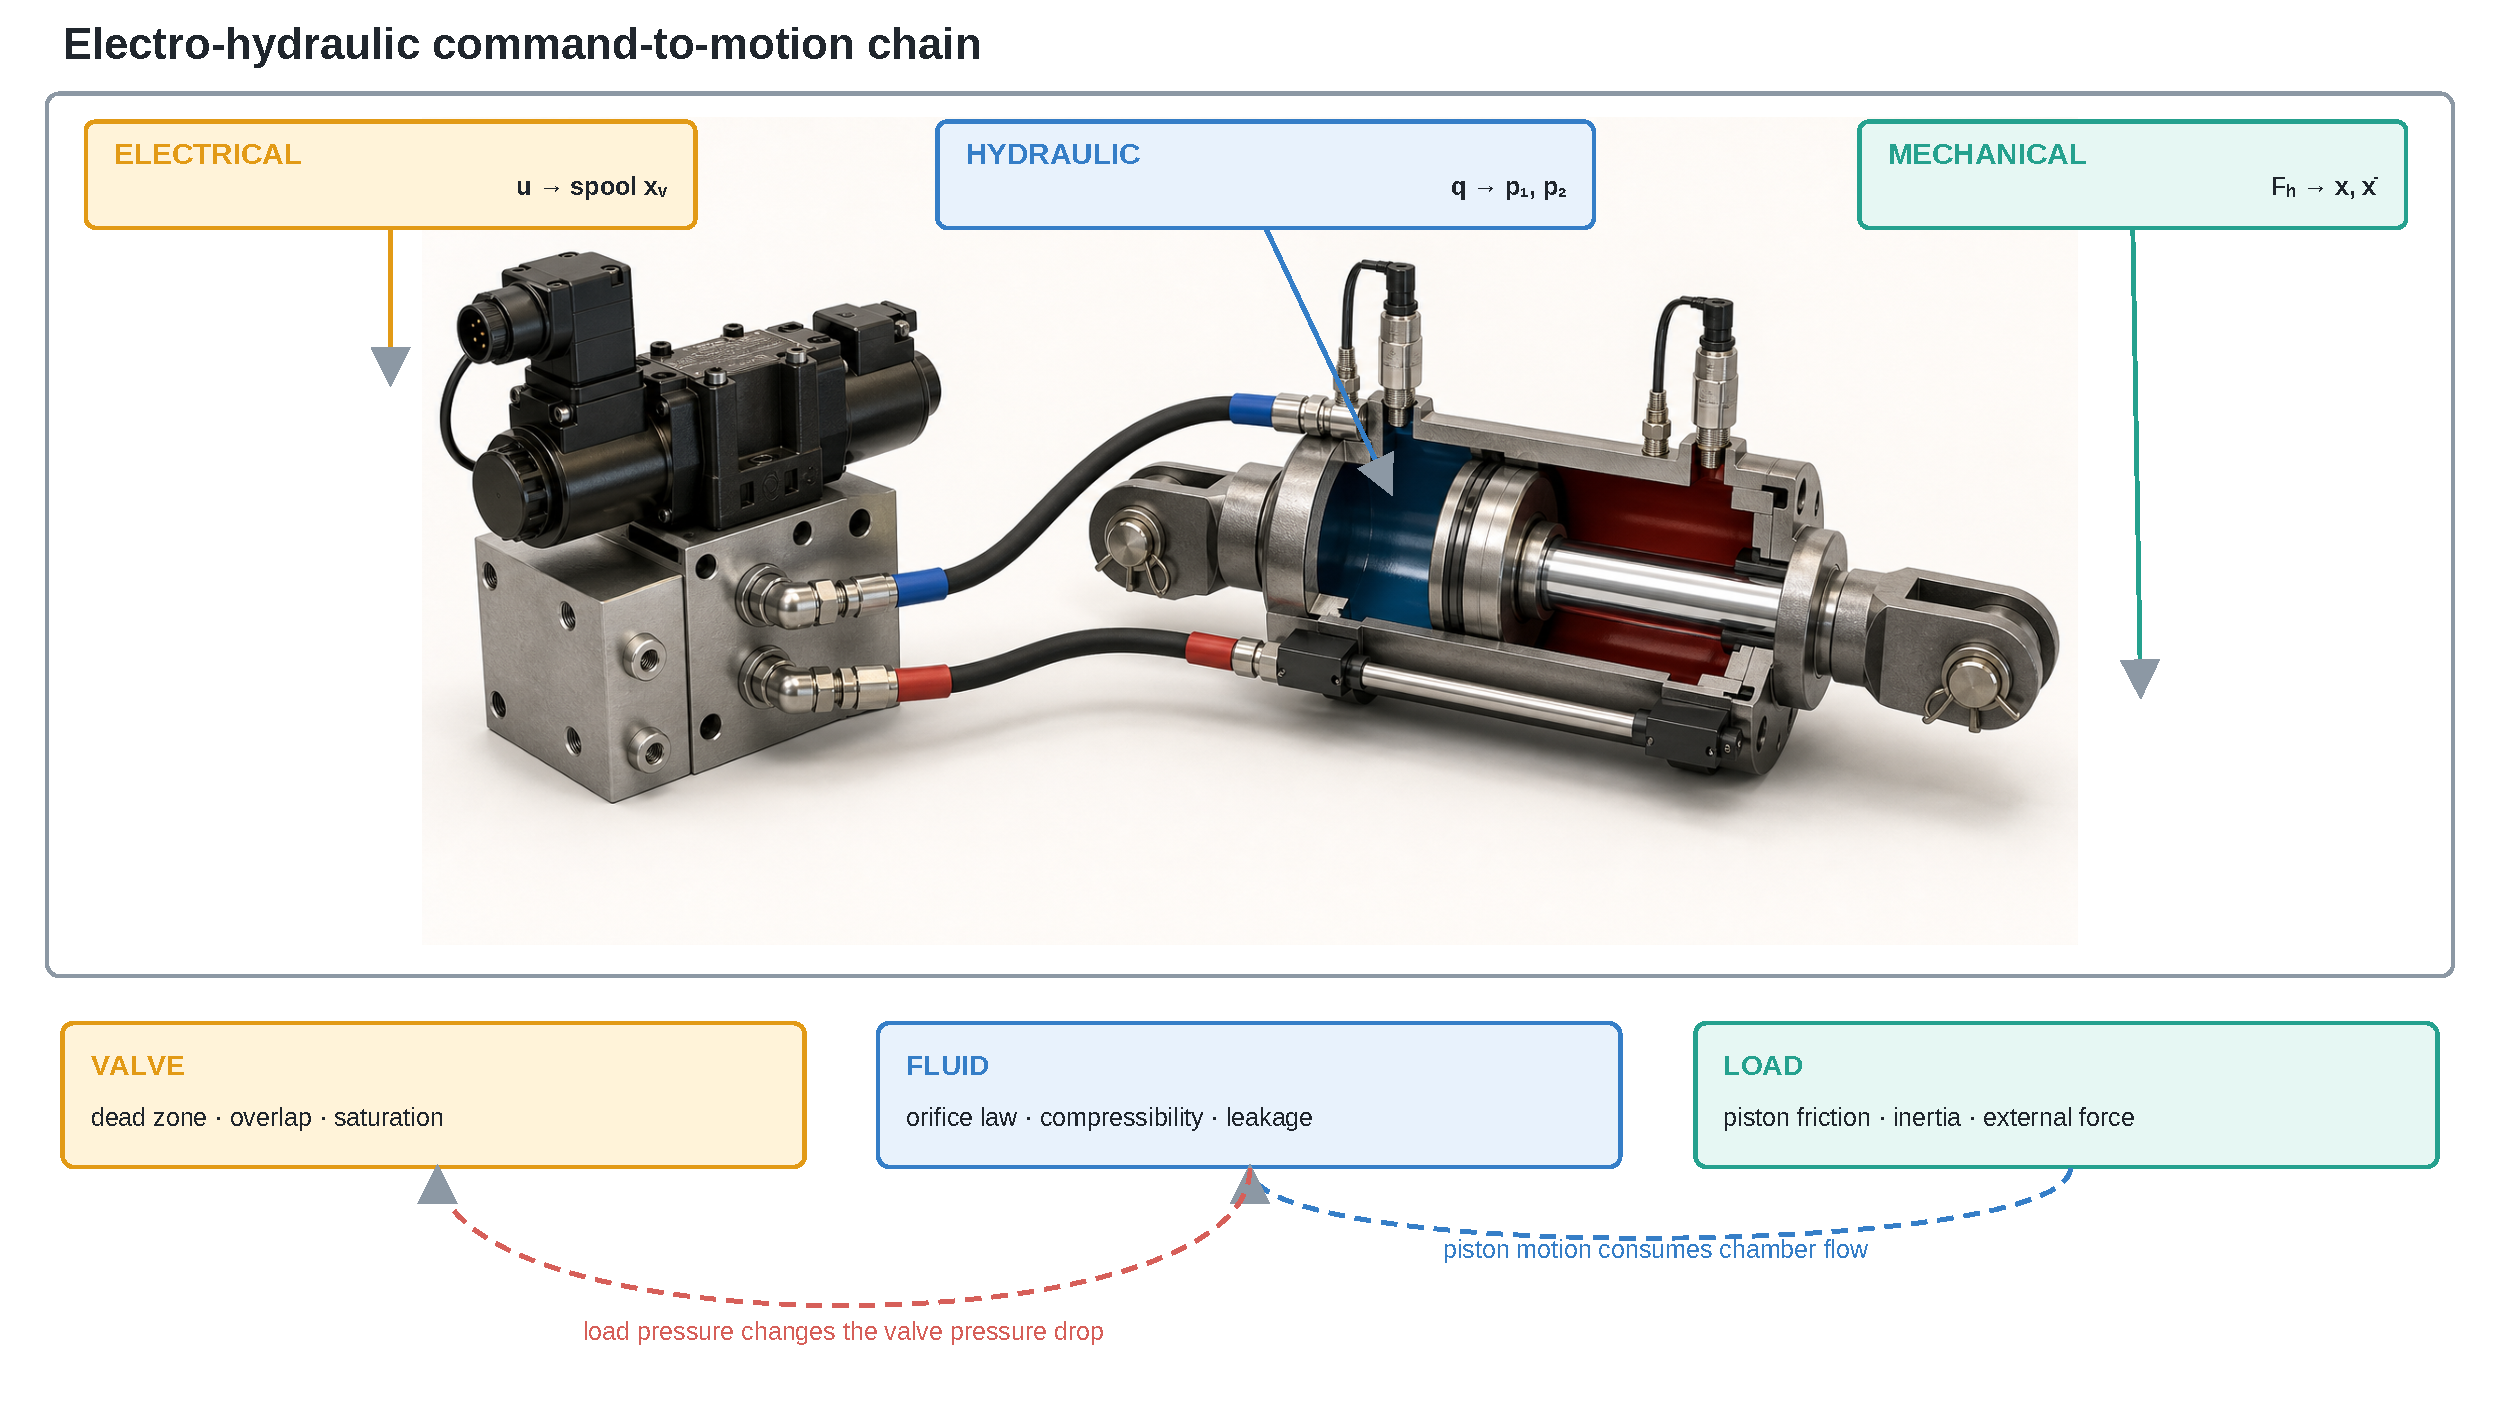
\includegraphics[width=\textwidth]{images/fund_actuation_chain}
  \caption{The electro-hydraulic actuation chain from valve command to
  mowing-head motion, grouped by energy domain. The tags beneath each
  domain name its dominant nonlinearities. The two dashed return paths
  are the physical feedback loops that make the effective gain of the
  chain an operating point rather than a constant: the load pressure
  throttles the valve flow through the square-root term of
  \eqref{eq:fund:orifice}, and the moving piston itself consumes flow
  before pressure can build.}
  \label{fig:fund:chain}
\end{figure}

Figure~\ref{fig:fund:chain} traces the signal path that every command to
the arm must traverse. A normalized electrical command displaces the
spool of a proportional valve, which opens metering orifices toward the
supply and tank lines. To first approximation, the resulting flow follows
the orifice law~\cite{merritt1967hydraulic}
%
\begin{equation}
  \label{eq:fund:orifice}
  q \;=\; c_d\, w\, x_v \sqrt{\tfrac{2}{\rho}\,\bigl|p_s - p_{\mathrm{load}}\bigr|}\;
  \operatorname{sgn}\bigl(p_s - p_{\mathrm{load}}\bigr),
\end{equation}
%
with discharge coefficient $c_d$, orifice area gradient $w$, spool
position $x_v$, oil density $\rho$, supply pressure $p_s$, and load
pressure $p_{\mathrm{load}}$. Two properties of \eqref{eq:fund:orifice}
shape everything that follows in this thesis. First, the flow gain
depends on the square root of the pressure margin. The same spool
displacement therefore moves the cylinder quickly under light load and
barely at all when the load pressure approaches supply. The effective
valve authority is an operating point, not a constant. Second, the
relation is directional. Extending against gravity and retracting with it
see different pressure margins and hence different gains. Around the
spool null, machining overlap produces a dead zone in which small
commands move nothing at all, and at the other end of the stroke the
spool saturates~\cite{jelali2003hydraulic}.

The delivered flow does not translate directly into motion either. Oil
is compressible, the more so when air is entrained, so each cylinder
chamber acts as a nonlinear spring. Its stiffness scales with the
effective bulk modulus and inversely with the chamber volume, and the
volume itself changes with piston position. Pressure relief valves clip
the dynamics whenever a load spike or an aggressive command drives a
chamber to its limit, which happens routinely in mowing when the head
rests on the ground. Internal leakage bleeds pressure between chambers,
seal friction opposes motion, and the load pressure feeds back into the
valve flow through \eqref{eq:fund:orifice}. Taken together, this is the
plant that the learned models of this thesis must represent: several
interacting nonlinearities, some of them non-smooth (relief, dead zone,
stiction), and parameters such as bulk modulus, leakage, and friction
that drift with temperature and wear.

One structural point matters for the control architecture. The chain in
Figure~\ref{fig:fund:chain} ends in the mechanical linkage, where
cylinder translation becomes joint rotation through lever arms that vary
with configuration. Uncertainty entering at the valve is therefore
filtered, amplified, and coupled by the mechanism before it appears as
head-position error. This is why the models of Chapter~\ref{chap:models}
are formulated in \emph{cylinder space}, directly across the hydraulic
conversion stages, rather than in task space where hydraulic and
kinematic effects blur together.

\subsection{High-Fidelity Simulation as a Data Source}
\label{sec:fund:sim-data-source}

The hydraulic subsystems above can be modeled in detail in
component-level simulation environments such as
Simscape~\cite{mathworks2024simscape}, and Chapter~\ref{chap:data} builds
on such a model of the FME~500 arm. It is tempting to close the loop and
train a reinforcement-learning policy directly against this model, but
the computational profiles do not match. The stiff pressure dynamics
force small integration steps, and the solver processes one machine
instance at a time, while modern policy optimization spreads its sample
cost over thousands of plants simulated in parallel on a
GPU~\cite{makoviychuk2021isaac}. This thesis resolves
the mismatch by separation: the high-fidelity model is used offline as a
data generator, and compact learned representations of the actuator
carry its behavior into the parallel training environment. How this
workflow fits together is shown later, in
Figure~\ref{fig:fund:workflow}, once its ingredients have been
introduced.

\section{Kinematics and Task-Space Tracking}
\label{sec:fund:kinematics}

\subsection{Differential Kinematics}

The mowing task is specified where the work happens, as a reference path
for the cutter in the coordinates of the vehicle. Task-space control
therefore rests on the differential kinematics of the
arm~\cite{siciliano2009robotics}. Writing $\bm{q}$ for the joint
configuration and $\bm{r}(\bm{q})$ for the forward-kinematic position of
the tool point, small motions are related through the manipulator
Jacobian $\bm{J}(\bm{q}) = \partial \bm{r} / \partial \bm{q}$,
%
\begin{equation}
  \label{eq:fund:diffkin}
  \dot{\bm{r}} = \bm{J}(\bm{q})\, \dot{\bm{q}} .
\end{equation}
%
Inverting \eqref{eq:fund:diffkin} to obtain joint or cylinder commands
from a desired tool velocity is the core of resolved-rate control. The
plain pseudoinverse solution is fragile. Near singular configurations,
which the mowing arm visits routinely (for instance with the boom almost
fully folded at the near edge of the envelope in
Figure~\ref{fig:fund:fme500}(b)), small task-space errors demand extreme
joint rates. The standard remedy, adopted unchanged in this thesis, is
the damped least-squares (DLS) inverse proposed independently by
Wampler~\cite{wampler1986manipulator} and by Nakamura and
Hanafusa~\cite{nakamura1986inverse}. It replaces the plain pseudo-inverse
with a damped one, trading a bounded amount of tracking accuracy for bounded
joint commands through a damping factor. The realization used in this thesis
is given in Section~\ref{sec:ctrl:dls}. DLS is conservative, well
understood, and cheap. These are the properties one wants in the layer of
the controller that must never misbehave.

\subsection{From Joint Space to Cylinder Space}

Equation~\eqref{eq:fund:diffkin} and the damped inverse are textbook
material for revolute arms. The complication on a hydraulic boom is that
the actuated coordinates are not the joint angles but the cylinder
lengths. Each cylinder closes a triangle over its joint, so the
cylinder-to-joint mapping is a configuration-dependent, monotone but
nonlinear relation, and its derivative, the lever arm, varies over the
stroke. Two practical consequences follow. First, the Jacobian used for control is the composition of the task Jacobian with the
joint-to-cylinder map, so that DLS can be solved directly for
cylinder-velocity commands. This thesis uses a calibrated $3{\times}4$
cutter-to-cylinder Jacobian identified on the simulated plant
(Chapter~\ref{chap:system}). Second, the mapping couples uncertainty: an
error in one cylinder's realized motion appears in the task error of the
whole arm, weighted by lever arms that change along the path. The FME~500
additionally has a passive fifth joint that is mechanically coupled to
the head, which constrains which task directions can be controlled
independently. Chapter~\ref{chap:system} works out the consequences.

The kinematic layer, however accurate, contains an assumption that this thesis does not make: that a commanded cylinder velocity is
a realized cylinder velocity. Everything in
Section~\ref{sec:fund:actuation-chain} argues against that assumption on
this actuator class. The kinematic controller is therefore treated as a
\emph{nominal} structure whose commands are realized, or not, by the
hydraulic layer. The learned models of this thesis live in that
realization gap.

\section{Model-Based and Conventional Control Approaches}
\label{sec:fund:conventional-control}

Industrial practice on machines like the FME~500 is open-loop operator
control: the joystick maps to valve current and the human closes every
loop. The control literature offers a spectrum of alternatives, none of which
alone settles the problem addressed here.

Classical cascade structures, an outer position loop commanding an inner
velocity or pressure loop with fixed PI or PD gains, are the workhorse of
hydraulic servo control~\cite{jelali2003hydraulic}. They are simple and
robust, but fixed gains must be tuned for the worst case across the
operating envelope, and Section~\ref{sec:fund:actuation-chain} showed
that the plant gain varies by an order of magnitude across that
envelope. The result is a controller that is sluggish where the plant is
weak or oscillatory where it is strong. On a boom whose lever arms change
with every meter of reach, one gain set cannot be right everywhere.

Model-based nonlinear methods attack the problem directly.
Computed-torque control cancels the rigid-body dynamics if they are
known~\cite{slotine1991applied}; backstepping
designs extend the idea through the pressure dynamics; adaptive versions
estimate uncertain parameters online~\cite{astrom1995adaptive}; robust
versions bound their effect. Applied to hydraulic manipulators, these
designs achieve impressive tracking in laboratory settings. Their
guarantees, however, are conditioned on structural model knowledge:
valve flow curves, friction models, inertia parameters. Obtaining and
maintaining that knowledge for a commercial implement, produced in
variants and operated across seasons, is expensive, and Mattila et
al.~\cite{mattila2017survey} conclude their survey with essentially this
observation: the accuracy of model-based hydraulic control is bounded by
the accuracy of the models, and the models are the bottleneck.

This thesis draws a specific lesson from that literature rather than
discarding it. Structured controllers are kept where structure is
reliable. The kinematic DLS layer of Section~\ref{sec:fund:kinematics}
is retained, because differential kinematics \emph{is} accurately known.
It serves as the privileged teacher that generates safe excitation and
supervises policy distillation, and as the closed-loop controller used
during identification data collection. Learning is directed at the part
where first-principles modeling is the bottleneck, the mapping between
cylinder-space commands and realized cylinder motion, and at the
task-level controller that issues those commands
(Section~\ref{sec:fund:rl-residual}). The architecture is hybrid by
design, not black-box.

\section{Data-Driven System Identification and Learned Dynamics}
\label{sec:fund:learned-dynamics}

\subsection{Learned Forward and Inverse Dynamics}

Where deriving a model is the bottleneck, one can measure it instead. In
robot model learning~\cite{nguyentuong2011model}, two complementary
mappings are distinguished. A \emph{forward dynamics} model predicts the
next state, or state increment, from the current state and the applied
command,
%
\begin{equation}
  \label{eq:fund:fd}
  \hat{\bm{s}}_{k+1} = \bm{s}_k + f_\theta(\bm{s}_k, \bm{u}_k),
\end{equation}
%
and an \emph{inverse dynamics} model predicts the command that realizes
a desired transition, $\bm{u}_k = g_\phi(\bm{s}_k, \bm{s}^{*}_{k+1})$.
Neural networks are the standard function class when the underlying
physics is non-smooth and history dependent, as it is here. For control,
one-step accuracy of \eqref{eq:fund:fd} is necessary but not
sufficient. A model used inside a planner or a training loop is iterated, feeding its
own prediction back as input, so small one-step errors compound over the
horizon. A model selected purely by one-step loss can diverge within a few
hundred milliseconds of recursive prediction~\cite{nagabandi2018neural}.
Multi-step rollout objectives, which iterate the model during training and
penalize the accumulated error, counteract this compounding directly and
are used for every dynamic model trained in this thesis. The
probabilistic-ensemble line of work~\cite{chua2018deep} addresses the
same problem by additionally tracking how model uncertainty grows along
the rollout. Where a single sample cannot summarize the relevant past,
for instance pressure transients and valve history, recurrent
architectures~\cite{hochreiter1997long,cho2014learning} extend
\eqref{eq:fund:fd} with an internal state that integrates a window of
history. The reduced-order model of Chapter~\ref{chap:models} takes this
form.

\subsection{Closed-Loop Identifiability}
\label{sec:fund:identifiability}

The dominant practical danger in learning \eqref{eq:fund:fd} is not
underfitting but learning the wrong thing well. System-identification
theory has long formalized when data determines a plant: informative
experiments require inputs that excite the dynamics independently of the
feedback law~\cite{ljung1999system,isermann2011identification}. Data
collected in closed loop violates this in a treacherous way. The
controller computes the command from the state history, so command and
state are strongly correlated, and a flexible model can reach excellent
prediction scores by exploiting the state history alone. It then behaves
like a sophisticated persistence model that ignores the input channel.
The failure is silent, because validation data from the same closed-loop
distribution keeps rewarding the shortcut. Schoukens and
Ljung~\cite{schoukens2019nonlinear} emphasize that for nonlinear systems
the design of informative excitation is, if anything, more critical than
for linear ones.

This is not a hypothetical concern in this thesis. It is a measured
event. The first forward-dynamics model of Chapter~\ref{chap:models},
trained on closed-loop operation data, reached one-step $R^2$ near
$0.999$ while an input ablation showed that it had learned almost no
dependence on the valve command at all. The open-loop excitation
campaign of Chapter~\ref{chap:data}, valve sequences applied directly
to the plant without any feedback controller in the loop, exists
specifically to break this correlation and make the causal
valve-to-motion path identifiable. The methodological rule that follows is applied to every
learned model in this work: input-ablation tests with zeroed and
shuffled commands are part of model acceptance, and a supervised score
is never accepted as evidence of control authority on its own.

\section{Reduced-Order Modeling}
\label{sec:fund:rom}

The term \emph{reduced-order model} comes from a large literature on
projecting high-dimensional dynamical systems onto low-dimensional
subspaces that preserve their dominant behavior. Benner et
al.~\cite{benner2015survey} survey this family, including parametric
variants that remain valid across a family of plants. The motivation is
the one that matters here: a model cheap enough to evaluate thousands of
times per second, yet faithful enough that conclusions drawn from it
transfer to the full system. This thesis uses the term in the same
spirit but with a learned construction. The full Simscape hydraulic
model, with its many internal states, is reduced to a compact
per-cylinder state (extension, extension velocity, pressure difference)
whose transition is learned from data.

Between white-box projection and black-box regression lies the grey-box
middle ground this thesis occupies. Physics-informed learning embeds
known structure, such as conservation laws or integrator chains, into
the hypothesis class, so that data is spent on what is unknown
rather than on rediscovering known
physics~\cite{karniadakis2021physics}. Lutter et
al.~\cite{lutter2019deep} demonstrated the benefit for rigid-body
dynamics by building Lagrangian structure into a network. The
reduced-order model of Chapter~\ref{chap:models} applies the same idea
to hydraulics: the orifice law \eqref{eq:fund:orifice}, the
pressure-buildup equation, and the velocity--position integrator chain
are explicit layers with trainable effective parameters, while neural
components supply only the valve realization, the
configuration-dependent load, and small bounded residuals. Two
properties motivated this choice over a free-form sequence model. The
trained effective parameters can be checked against physical
plausibility, and the bounded residuals mean that even an
off-distribution input cannot produce an unphysical state jump. A
policy-training loop, which pushes its model off-distribution by design,
benefits from both.

The closest precedent for embedding such a surrogate in policy training
comes from legged robotics. Hwangbo et
al.~\cite{hwangbo2019learning} identified the rigid-body mechanics of
their robot analytically, learned the response of its series-elastic
actuators from measured data, trained a policy against the resulting
hybrid simulation, and deployed it directly on the machine. Later work
industrialized this recipe in GPU-parallel
simulators~\cite{rudin2022learning}. The premise has since been
inverted as well: Yamamori et al.~\cite{yamamori2026actuator} shape the
closed-loop response of the physical actuator to match the idealized
dynamics assumed in simulation, so that the model is met by the hardware
rather than the hardware by the model. That option is unavailable here,
because the valve and pump of a commercial implement carrier are not
open to redesign, which is precisely why the modeling burden in this
thesis falls on the actuator representation.
Figure~\ref{fig:fund:workflow}
shows how this thesis adopts the same division of labor with the roles
recast for hydraulics. The PhysX articulation in IsaacLab plays the
analytic rigid-body part, and the learned part is not a torque filter
for a well-behaved electric drive but the entire hydraulic chain of
Figure~\ref{fig:fund:chain}. That difference is why the surrogate here
must be hydraulic-aware, structured around pressure dynamics and valve
nonlinearity, and command-conditioned, so that it realizes desired
cylinder commands on the plant side rather than filtering torques.

\begin{figure}[tb]
  \centering
  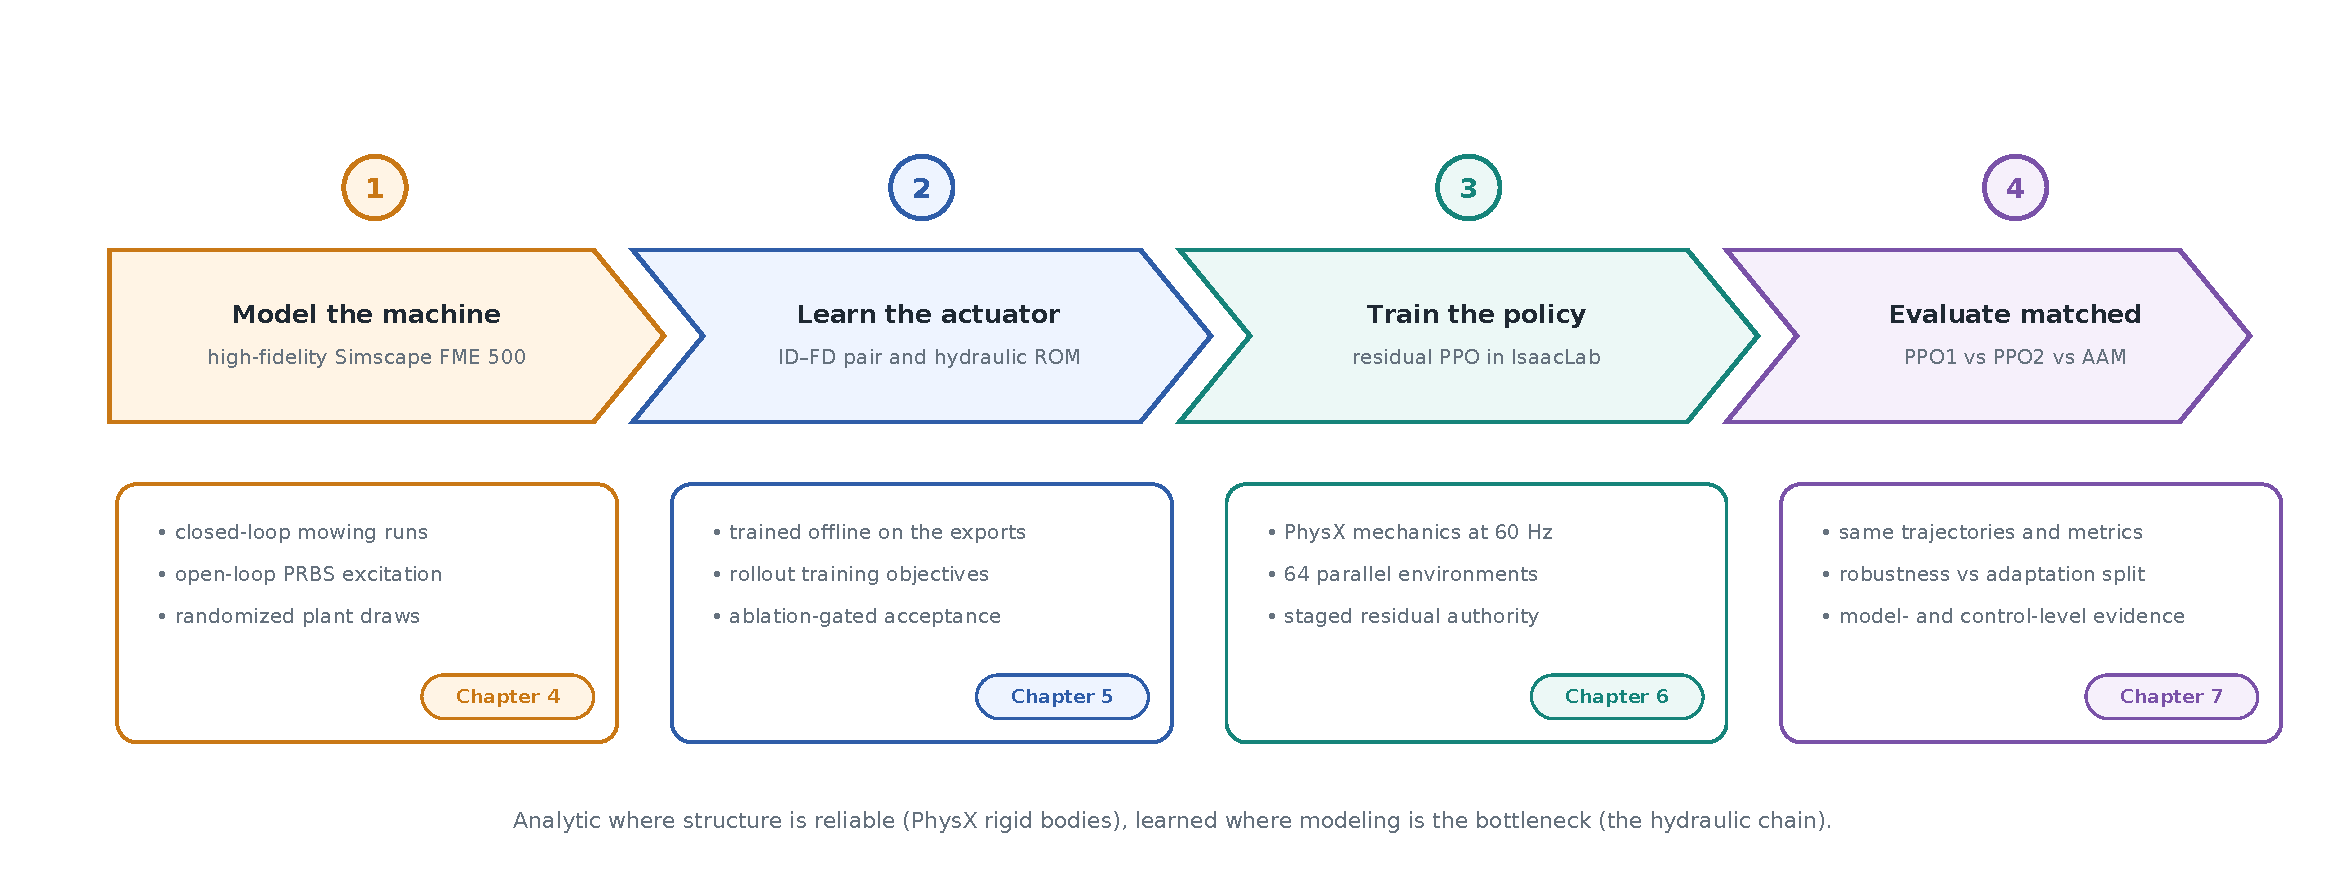
\includegraphics[width=\textwidth]{images/fund_workflow}
  \caption{The four-step workflow of this thesis, following the division
  of labor introduced for legged robots by Hwangbo et
  al.~\cite{hwangbo2019learning}: model what is reliably known, learn
  the actuator from data, train the policy against the combination, and
  evaluate under matched conditions. The cards list what each step
  contributes and the chapter that develops it.}
  \label{fig:fund:workflow}
\end{figure}

\section{Domain Randomization and Latent Adaptation}
\label{sec:fund:domain-randomization}

\subsection{Robustness Through Randomized Training}

A model or policy trained on one simulated plant inherits every
parameter of that plant as an implicit assumption. Domain randomization
attacks this brittleness by training across a distribution of plants,
originally over visual appearance for
perception~\cite{tobin2017domain}, soon after over dynamics parameters
such as masses, frictions, gains, and latencies for
control~\cite{peng2018sim}. The now-standard reading of those results is
that a policy or model that must succeed on many plants converges to
behavior that is \emph{robust} across the family. For the hydraulic arm
the corresponding family is physically meaningful rather than
synthetic: effective bulk modulus varies with entrained air and
temperature, valve gains and leakage drift with wear, and payload
changes with the mounted attachment. Chapter~\ref{chap:data} defines the
randomized parameter space along these same axes.

\subsection{From Robustness to Adaptation}

\begin{figure}[tb]
  \centering
  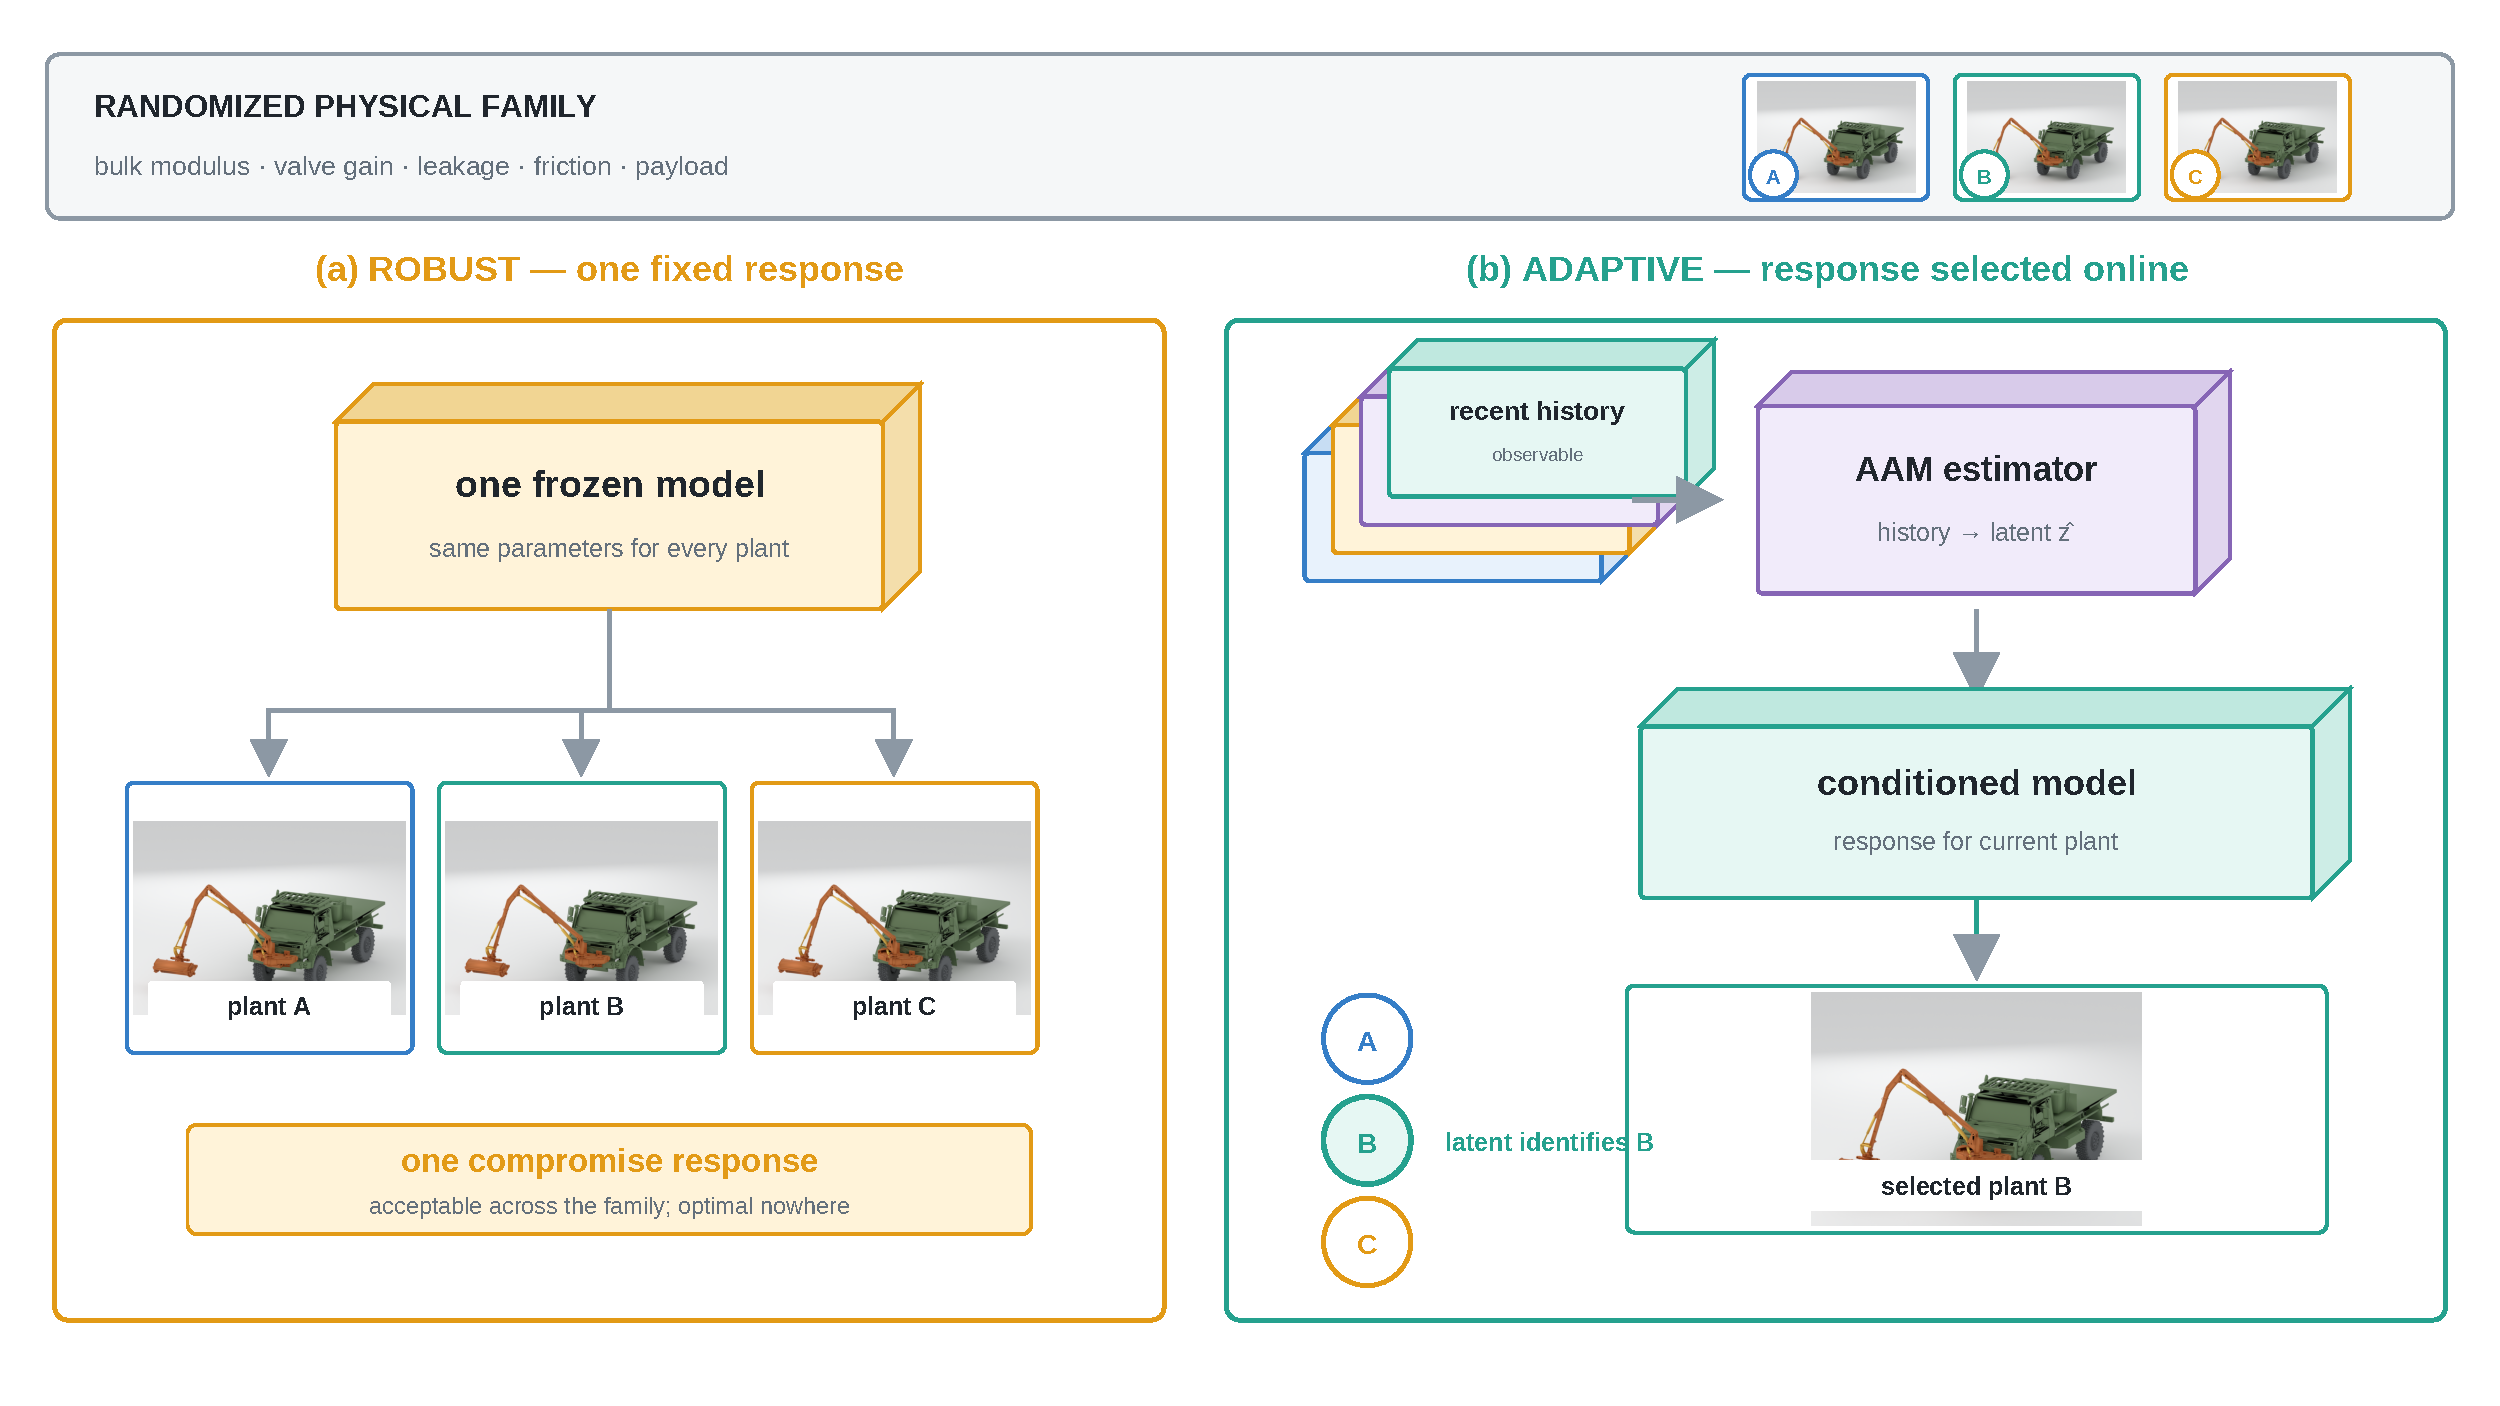
\includegraphics[width=\textwidth]{images/fund_robust_adaptive}
  \caption{The distinction this thesis is built to measure, as two
  treatments of the same randomized plant family. (a)~Randomized
  training alone produces a \emph{robust} model: one fixed response
  that works acceptably everywhere and optimally nowhere. (b)~Latent
  conditioning adds \emph{adaptation}: an estimator infers a compact
  representation $\hat{\bm{z}}$ of the currently active plant from
  recent measured history, and the downstream model or controller
  changes its response accordingly. The estimator is trained against a
  privileged latent computed from the true physical factors
  $\factorvec$, but deploys on observable measurements alone.}
  \label{fig:fund:robust-adaptive}
\end{figure}

Robustness, however, is a compromise by definition: one response that is
acceptable everywhere is optimal nowhere. The alternative is to let the
controller or model identify which member of the family it is currently
facing and condition on that estimate
(Figure~\ref{fig:fund:robust-adaptive}). The teacher--student
construction makes this trainable. During simulation the true randomized
factors $\factorvec$ are known, and a privileged encoder compresses
them, or their dynamic consequences, into a low-dimensional latent
$\bm{z}$. A
student module then learns to regress $\bm{z}$ from signals that exist
outside simulation, namely the recent history of states, commands, and
responses. Lee et al.~\cite{lee2020learning} used this scheme to walk
over terrain whose properties the robot cannot observe directly. Kumar
et al.~\cite{kumar2021rma} sharpened it into rapid motor adaptation:
a first phase trains the policy together with an encoder of the
privileged environment parameters, a second phase trains an adaptation
module to recover the same latent from the observable state--action
history, and at deployment only the history-based estimate is used, so
the system adapts within fractions of a second without any gradient
updates. Classical adaptive control pursues the same goal through online
parameter estimation~\cite{astrom1995adaptive}. The learned variant
replaces explicit parameter estimates with a task-shaped latent, trading
physical interpretability for the ability to summarize many interacting
parameters at once. The construction has since been carried into the
dynamics model itself rather than the policy. Yu et
al.~\cite{yu2026context} condition a neural-ODE dynamics model on a
context vector inferred from state--action history, so the learned model
rather than the controller is what adapts to the current plant. That is
the position the AAM occupies here, and the reason this thesis measures
the adaptation effect at the actuator layer instead of inside the
policy.

The Arm Adaptation Module (AAM) of this thesis
(Chapter~\ref{chap:models}) is this construction applied to hydraulic
actuation, following the adaptive path of
Figure~\ref{fig:fund:robust-adaptive}(b). The privileged latent
$\bm{z} = \mu(\factorvec)$ is a two-dimensional compression of the
physical factor vector $\factorvec$, validated by the system-dynamics
surrogate of Chapter~\ref{chap:models}. The AAM reads its deployable
estimate $\latenthat$ from a quarter second of causal, observable
cylinder-signal history.

Where that estimate is \emph{used} is a design decision that this thesis
fixes explicitly, because it is easy to state loosely. The latent does
not condition the reduced-order model. In the proposed stack,
\ppoIDAAMFD, the inferred latent conditions a small bounded residual
adapter around the \emph{frozen inverse-dynamics model}, leaving the
forward model, the policy, and the PhysX plant unchanged. Conditioning
the policy directly on $\latenthat$ is treated as an ablation rather
than the default design (Chapter~\ref{chap:evaluation}). Two claims are
therefore kept apart throughout. A model trained across randomized
plants is \emph{robust}, not automatically adaptive, and evidence that a
\emph{privileged} latent carries useful dynamics information is not
evidence that an \emph{inferred} one improves control. Collapsing either
pair is a common confound in the sim-to-real literature, and the
experimental design of Chapter~\ref{chap:evaluation} is built to avoid
both.

\section{Reinforcement Learning and Structured Priors}
\label{sec:fund:rl-residual}

\subsection{Policy Optimization}

Reinforcement learning frames control as sequential decision making: a
policy $\pi_\vartheta(\bm{a}\,|\,\bm{o})$ maps observations to actions
and is optimized to maximize expected cumulated
reward~\cite{sutton2018reinforcement}. Among policy-gradient methods,
proximal policy optimization (PPO)~\cite{schulman2017proximal} has
become the default in robot learning for its simplicity and stable
large-batch behavior. It constrains each update through a clipped surrogate objective, which
limits how far the ratio between the new and the old policy may move before
the improvement term stops paying. Advantages are estimated with generalized
advantage estimation~\cite{schulman2016gae}. The objective as configured for
this thesis is written out in Section~\ref{sec:ctrl:optimization}. What makes
on-policy methods like PPO practical for this thesis is throughput.
GPU-parallel simulators run thousands of environment instances at
once~\cite{makoviychuk2021isaac}, and locomotion policies have been
trained this way in minutes~\cite{rudin2022learning}. This is the regime
in which the full hydraulic model cannot run
(Section~\ref{sec:fund:sim-data-source}) and the learned actuator
surrogates can.

\subsection{Structured Priors for Policy Learning}
\label{sec:fund:prior}

Applying RL to the mowing arm from scratch would discard the reliable
kinematic structure of Section~\ref{sec:fund:kinematics} and force the
policy to rediscover it from reward, slowly and with excursions that a
heavy boom cannot afford. Two established constructions inject that
structure, and they differ in \emph{where} the classical controller
appears at deployment.

Residual reinforcement learning adds the policy output to the command of a
hand-designed controller at
runtime~\cite{johannink2019residual,silver2018residual}, with the policy
restricted to a small bounded band. The nominal controller therefore provides
competent behavior from the first step, and exploration happens in a narrow
neighbourhood around it. The nominal controller remains in the deployed loop, and every
result is a property of the pair.

Policy distillation moves the same prior to training time instead. A
privileged teacher, here the DLS controller, which may read
quantities the deployed system cannot, generates demonstrations, and
the student policy is fitted to them by supervised imitation before any
reward is optimized~\cite{ross2011reduction}. At deployment the teacher
is gone: the student is the whole controller.

A third construction, used for the final policies of this thesis and
developed in Section~\ref{sec:ctrl:anchored}, keeps the prior for the
whole of optimization without returning it to the runtime loop. The
distilled student is frozen as a \emph{reference} policy, and reward
optimization is then restricted to a neighbourhood of it, measured as a
divergence between the two action distributions. The reference is queried only
on states the learner itself visits and never supplies an executed action. The
constraint is stated formally in Section~\ref{sec:ctrl:anchored}.
The three constructions are therefore distinguished by \emph{when} the prior
acts: at every runtime step, at initialization only, or throughout
optimization as a constraint. Only the first leaves a classical
controller inside the deployed loop.

This thesis uses the second and third constructions, and the distinction
from the first is not cosmetic. The deployed policy of all three stacks is a \emph{sole}
cylinder-motion controller: it emits the desired cylinder command
itself, with no nominal command added to its output at runtime. The DLS
controller is retained as the privileged teacher for distillation and as
the closed-loop controller during identification data collection, not as
a runtime layer. What bounds exploration is therefore not a residual band around a nominal
command but the action contract itself, which keeps commanded motion
inside the learned actuator's validated envelope and is specified in
Chapter~\ref{chap:control}.

The question of how to improve a policy that a simulator has already
made competent is active in its own right. Yin et
al.~\cite{yin2025rapidly} keep the value function learned in simulation
and use it to guide exploration during real-world fine-tuning, which
treats the simulator as a source of structure rather than as a plant to
be abandoned once training ends. The construction of this thesis shares
that premise and differs in what is retained: not the value function but
the policy itself, held as a fixed reference that bounds how far reward
optimization may travel.

One result of this thesis is reported here because it is what motivates
the third construction rather than a design assumption that precedes it.
In the maintained pipelines, \emph{unconstrained} PPO fine-tuning from
the distilled student raised total reward while degrading the primary
tracking objective, and did so consistently enough that distillation was
for several development cycles treated as the \emph{endpoint} rather
than an initialization. The diagnosis is a mismatch of objectives rather
than a failure of the optimizer: the reward is a proxy, acceptance is
decided by a set of physical gates, and the reward's optimum does not
lie inside the gate-feasible set (Section~\ref{sec:ctrl:training}).
The anchored construction is the response to that finding, and
it is what allows the reported \ppoROM{} policy of
Chapter~\ref{chap:control} to be a fine-tuned actor rather than a
distilled one.

\subsection{Reinforcement Learning on Hydraulic Machines}

Applications of deep RL to hydraulically actuated arms are still few,
and the closest of them sharpen rather than close the gap this thesis
addresses. Egli and Hutter demonstrated RL-based trajectory tracking for
the arm of a full-size hydraulic excavator, first in
simulation-to-machine transfer experiments~\cite{egli2020towards} and
then as a general automation approach deployed on a walking
excavator~\cite{egli2022general}. Spinelli et
al.~\cite{spinelli2024rl} extended that line to material handlers whose
tool is underactuated, training in simulation and validating on a
commercial machine, which shows the approach scales to arms where part
of the mechanism is not directly commanded. The mowing head of this
thesis is underactuated in the same sense, through its passive swivel
joint. Maitan et al.~\cite{maitan2026contraction} attacked the problem
from the opposite end, learning force control for a single hydraulic
actuator directly on hardware and constraining exploration with a
contraction-metric filter so that training on a real cylinder stays
safe. Their work is the closest published statement of the difficulty
this thesis handles in simulation: an unconstrained policy acting on a
hydraulic cylinder is not safe by default, and something must bound it.
Their key ingredient is shared with
this work: a data-driven model of the machine's actuator response,
learned from recorded operation and used as the training plant for the
policy. The differences define where this thesis stands. Their actuator
model is identified for one physical machine, so robustness across a
plant family and online adaptation to a changing plant are outside its
scope. Their policy is trained against that single model without a
privileged teacher supplying the structured prior. And their evaluation
compares against human operators and classical baselines rather than
isolating the contribution of the actuator representation itself. The
comparison that Chapter~\ref{chap:evaluation} is built around (same task, same policy architecture, same observation and action contracts,
same terrain, reward, seeds and training budget, with only the actuator and adaptation path differing) has to the author's knowledge no
published counterpart for hydraulic manipulators.

One property of a learned policy over a learned actuator cuts both ways
and shapes the evaluation methodology of this thesis. Because the policy
can compensate for a mediocre actuator model, closed-loop tracking error
alone cannot distinguish a good model from a good patch over a bad one.
The protocol of Chapter~\ref{chap:evaluation} therefore reports
model-level rollout metrics, the magnitude and smoothness of the emitted
commands, and the standing cylinder-tracking and actuator-prediction
residuals alongside task error. A better actuator representation must show up as a smaller standing model error and
quieter commands, not merely as equal tracking.

\section{Research Gap and Thesis Positioning}
\label{sec:fund:gap}

Laid side by side, the threads of this chapter each solve part of the
problem and leave a specific remainder
(Table~\ref{tab:fund:positioning} names the works). Hydraulic control
theory provides structure and explains why fixed models fail, but its
precise methods presuppose plant knowledge that a commercial mowing
implement does not come with. Learned dynamics models replace
derivation with data, but the identifiability literature, and the
measured failure recounted in Section~\ref{sec:fund:identifiability},
shows that closed-loop operation data silently produces models without
control authority. Learned actuator surrogates embedded in parallel
simulation are proven for electric drives but not for actuators
dominated by pressure dynamics, relief saturation, and valve dead
zones. Domain randomization yields robustness, and the teacher--student
construction yields fast online adaptation, but these results live
almost entirely in locomotion, where the adapted quantity is the
contact with the world rather than the actuator itself. RL has reached
full-size hydraulic arms, but without a structured prior, without
adaptation, and without isolating the actuator representation.
Residual RL and policy distillation both integrate learning with a
structured controller, yet published evaluations rarely control for the
fact that the policy can mask actuator-model deficiencies.

\begin{table}[tb]
  \centering
  \caption{Positioning of this thesis against the reviewed lines of work.
  Columns: (I)~learned model of \emph{hydraulic} actuator dynamics;
  (II)~training data audited for causal input identifiability;
  (III)~online latent adaptation to a changing plant; (IV)~structured
  classical controller retained as a prior, with bounded action
  authority; (V)~matched comparison isolating the actuator
  representation.
  ($\checkmark$)~=~partially or implicitly addressed.}
  \label{tab:fund:positioning}
  \small
  \begin{tabular}{lccccc}
    \toprule
    Line of work & I & II & III & IV & V \\
    \midrule
    Model-based hydraulic control~\cite{mattila2017survey,jelali2003hydraulic}
      & --- & ($\checkmark$) & ($\checkmark$) & $\checkmark$ & --- \\
    Actuator networks for legged robots~\cite{hwangbo2019learning,rudin2022learning}
      & --- & $\checkmark$ & --- & --- & --- \\
    RL for hydraulic excavators~\cite{egli2020towards,egli2022general}
      & $\checkmark$ & ($\checkmark$) & --- & --- & --- \\
    Locomotion adaptation~\cite{lee2020learning,kumar2021rma}
      & --- & --- & $\checkmark$ & --- & --- \\
    Residual RL and policy
    distillation~\cite{johannink2019residual,silver2018residual,ross2011reduction}
      & --- & --- & --- & $\checkmark$ & --- \\
    \midrule
    This thesis (\ppoROM{} / \ppoIDFD{} / \ppoIDAAMFD)
      & $\checkmark$ & $\checkmark$ & $\checkmark$ & $\checkmark$ & $\checkmark$ \\
    \bottomrule
  \end{tabular}
\end{table}

What is missing is the combination, summarized in
Table~\ref{tab:fund:positioning}: cylinder-space actuator dynamics
learned from deliberately identifiable data; a compact,
physics-structured, command-conditioned reduced model of those dynamics
that can run in massively parallel policy training; a compact dynamics
latent whose usefulness is demonstrated before it is deployed, together
with an online estimator that recovers it from observable history alone
and feeds a bounded correction into the actuator path; and a task-space
control framework in which adaptive and non-adaptive actuator
representations are compared under matched conditions, with model-level
and control-level evidence kept separate.

Assembling and evaluating this combination on the MULAG FME~500
mowing arm is the contribution of this thesis, and it takes the form of
three control stacks that differ \emph{only} in the actuation and
adaptation path between the policy's cylinder command and PhysX:

\begin{description}
  \item[\ppoROM.] The policy commands desired cylinder motion, which the
    validated command-conditioned reduced-order model realizes. This is
    the certified actuator baseline and the current shippable stack.
  \item[\ppoIDFD.] The same policy interface drives the frozen inverse
    model followed by the validated strict forward model. This is the
    non-adaptive learned baseline. It tracks the line more finely than
    \ppoROM{} and fails the ground-contact requirement, which makes it an informative negative result rather than a weaker copy.
  \item[\ppoIDAAMFD.] The AAM infers a dynamics latent from causal
    observable history, and that latent conditions a small bounded
    residual adapter around the frozen inverse model before the same
    frozen forward model and PhysX. This is the proposed adaptive
    method.
\end{description}

The scientific variable in the final comparison is therefore the
actuator and adaptation path alone. Task, observation and action
contracts, terrain, reward, training budget, test factors, seeds and
acceptance gates are held matched. Robustness (training across a
randomized plant family) and adaptation (conditioning on an inferred
estimate of the plant currently in front of the controller) are measured
as separate effects rather than conflated ones.

The next chapter grounds this program in the concrete system: the
simulated FME~500 plant, its coordinate spaces and measured signals, the
verge-following task, the control architecture, and the formal statement
of the tracking, robustness, and adaptation objectives.
